% MGD (Monitor-Guided Decoding) workflow figure.
% Synchronous LSP query at every '.' trigger; tokens outside the
% suggestion set are masked to -infinity. Block decoding semantics.
\documentclass[border=2pt]{standalone}
\usepackage{tikz}
\usepackage{xcolor}
\usetikzlibrary{shapes.geometric, arrows.meta, positioning, fit, backgrounds, calc}

\begin{document}
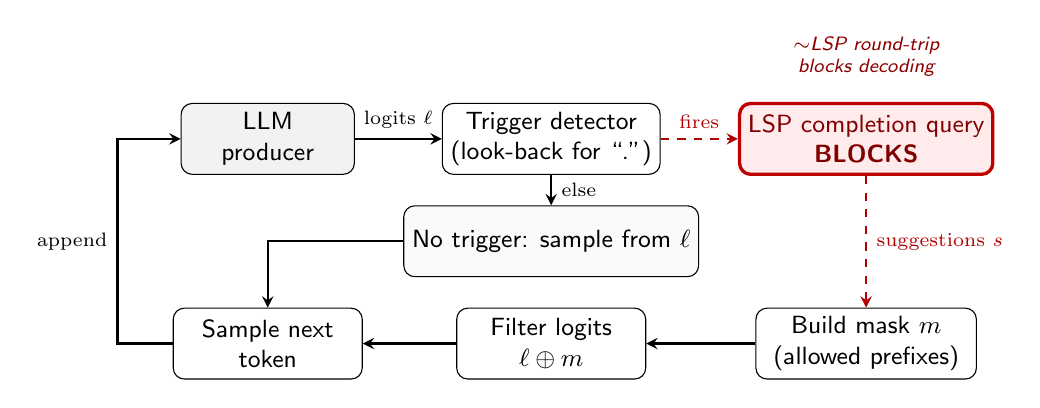
\begin{tikzpicture}[
    >=stealth,
    font=\sffamily\small,
    box/.style       ={draw, rounded corners, align=center, minimum height=9mm,
                       minimum width=24mm, inner sep=3pt, fill=white},
    llmbox/.style    ={box, fill=black!5, minimum width=22mm},
    blockbox/.style  ={box, draw=red!75!black, very thick, fill=red!8,
                       text=red!50!black, minimum width=28mm},
    flow/.style      ={->, thick},
    blockflow/.style ={->, thick, red!70!black, dashed},
    note/.style      ={font=\sffamily\scriptsize\itshape, text=red!55!black}
]

% Top row: producer -> trigger -> LSP
\node[llmbox] (llm) at (0,0) {LLM\\producer};
\node[box]      (trig) at (3.6,0) {Trigger detector\\(look-back for ``.'')};
\node[blockbox] (lsp)  at (7.6,0) {LSP completion query\\\textbf{BLOCKS}};

% Annotation above LSP
\node[note, above=2mm of lsp, text width=34mm, align=center]
    {$\sim$LSP round-trip\\blocks decoding};

% Bottom row: sample <- filter <- mask
\node[box, minimum width=28mm] (mask) at (7.6,-2.6) {Build mask $m$\\(allowed prefixes)};
\node[box]   (filt) at (3.6,-2.6) {Filter logits\\$\ell \oplus m$};
\node[box]   (samp) at (0,-2.6)   {Sample next\\token};

% Wait-branch (no trigger) placed slightly off the main path
\node[box, fill=black!2, minimum width=28mm, align=center]
    (wait) at (3.6,-1.3) {No trigger: sample from $\ell$};

% --- Arrows ---
\draw[flow] (llm.east) -- (trig.west)
    node[midway, above, font=\scriptsize] {logits $\ell$};
\draw[blockflow] (trig.east) -- (lsp.west)
    node[midway, above, font=\scriptsize] {fires};
\draw[blockflow] (lsp.south) -- (mask.north)
    node[midway, right, font=\scriptsize] {suggestions $s$};
\draw[flow] (mask.west) -- (filt.east);
\draw[flow] (filt.west) -- (samp.east);

% Wait branch: trig -> wait -> samp
\draw[flow] (trig.south) -- (wait.north)
    node[midway, right, font=\scriptsize] {else};
\draw[flow] (wait.west) -| (samp.north);

% Loop back: samp -> llm
\draw[flow] (samp.west) -- ++(-7mm,0) |- (llm.west)
    node[pos=0.25, left, font=\scriptsize] {append};

\end{tikzpicture}
\end{document}
